\chapter{光学系统中光束的限制}

\begin{introduction}
	\item 孔径光阑(第 \ref{subsect:aperture-stop} 节)
	\item 视场光阑(第 \ref{subsect:field-stop} 节)
	\item 渐晕光阑(第 \ref{subsect:vignetting-stop} 节)
	\item 景深(第 \ref{sect:depth-of-field} 节)
\end{introduction}

\section{光阑}
\subsection{孔径光阑}
\label{subsect:aperture-stop}
\begin{definition}{孔径光阑}{aperture-stop}
在一个光学系统的若干通光孔中,有一个光孔起着限制成像光束(孔径角)的作用。这个光孔就是系统的孔径光阑。严格地说,限制轴上物点孔径角$u$的大小,限制轴上物点成像光束宽度、并有选择轴外物点成像光束位置作用的光阑叫做孔径光阑。
\end{definition}

孔径光阑可以安放在透镜前、透镜上、透镜后,三个位置对\textbf{轴上物点}光束宽度的限制作用是一样的。对于\textbf{轴外物点}参与成像的光束,孔阑位置不同,轴外物点参与成像的光束位置也不同。孔阑位于透镜上时,为使所有轴上物点和轴外物点发出的光束均参与成像所需的透镜口径是最小的。

光瞳是孔径光阑的像。孔径光阑经孔阑前面光学系统所成的像为入射光瞳,经孔阑后面光学系统所成的像为出射光瞳。

孔径光阑、入瞳、出瞳三者互为物像关系。孔阑在系统最前方,系统的入瞳与孔阑重合,孔阑本身就是入瞳;孔阑安放在透镜上,若透镜可当薄透镜处理,则孔阑本身是系统的入瞳和出瞳;孔阑在系统的最后方,系统的出瞳与孔阑重合,孔阑本身为出瞳。

\begin{problem}
	已知照相物镜的焦距为$50\mathrm{mm}$,相对孔径$D/f'=1/4$,入瞳到出瞳的放大率为$\beta_p=1.2$,求出瞳的直径。 
	\begin{tasks}(6)
		\task $12.5\mathrm{mm}$
		\task $200\mathrm{mm}$
		\task $15\mathrm{mm}$
		\task $240\mathrm{mm}$
		\task $10.43\mathrm{mm}$
		\task $166.67\mathrm{mm}$
	\end{tasks}
\end{problem}
\begin{solution}
	选择c。
\end{solution}

\subsection{视场光阑}
\label{subsect:field-stop}
实际光学系统中,物面上发出并进入系统参与成像的光束宽度是有限的,能够清晰成像的物面大小也是有限的。把能够清晰成像的物面范围称为光学系统的物方视场。相应的像面范围为像方视场。

\begin{definition}{视场光阑}{field-stop}
	在物面或像面上安放一个光阑,光阑的大小限定了物面或者像面的大小,即光学系统的成像范围。这个限定成像范围的光阑为视场光阑。
\end{definition}

视场光阑经其前面的光学系统所成的像称为入射窗,经其后面的光学系统所成的像称为出射窗。如果视场光阑安放在物平面上,则入射窗就是视场光阑,出射窗与像平面重合。入射窗、视场光阑、出射窗三者互为物像关系。

\subsection{渐晕光阑}
\label{subsect:vignetting-stop}
\begin{definition}{渐晕光阑}{vignetting-stop}
轴外点和轴上点需要通光全部成像光束的透镜口径大小不一样,轴外点光束部分光被透镜边缘阻挡而不能参与成像,导致轴外点成像光束宽度较轴上点成像光束宽度小,因此像平面边缘比像面中心暗,这种现象就是渐晕,透镜的边缘起拦光作用,为渐晕光阑。
\end{definition}

光孔离孔阑越远,越容易引起渐晕。一般以渐晕系数描述光束渐晕的程度。面渐晕系数是轴外点成像光束在入(出)瞳面上的截面积与入(出)瞳面积之比,线度之比为线渐晕系数。

\begin{figure}[htbp]
	\centering
	\begin{tikzpicture}[scale=0.9] 
	%\coordinate [label=above left:$P$] (A) at (-1,1);
	\coordinate [label=above right:$P_1$] (A) at (-1,1);
	\coordinate [label=below right:$P_2$] (B) at (-1,-1);
	\coordinate [label=below right:$P$] (C) at (-1,0);
	\coordinate [label=above left:$M_1$] (D) at (-3,1.2);
	\coordinate [label=above left:$M_2$] (E) at (-3,-1.2);
	\coordinate [label=above left:$M$] (F) at (-3,0);
	\coordinate [label=left:$A$] (G) at (-6,0);
	\coordinate [label=left:$B_1$] (H) at (-6,-1.5);
	\coordinate [label=left:$B_2$] (I) at (-6,-3);
	\coordinate [label=left:$B_3$] (J) at (-6,-4.5);
	\coordinate [label=right:$2a$] (K) at (-1,0.6);
	\draw[-] (-6,0) -- (0,0);
	\draw[-] (-6,2.4) -- (-6,-4.8);
	\draw[-,blue] (-6,0) -- (A);
	\draw[-,blue] (-6,0) -- (B);
	\draw[-,cyan] (-6,-1.5) -- (A);
	\draw[-,cyan] (-6,-1.5) -- (B);
	\draw[-,violet] (-6,-3) -- (A);
	\draw[-,violet] (-6,-3) -- (B);
	\draw[-,violet] (-6,-3) -- (C);
	\filldraw[violet,pattern=north east lines,pattern color=violet] (-6,-3) -- (B) -- (C) -- (-6,-3);
	\draw[-,red] (-6,-4.5) -- (A);
	\draw[-,red] (-6,-4.5) -- (B);
	\filldraw[red,pattern=north west lines,pattern color=red] (-6,-4.5) -- (A) -- (B) -- (-6,-4.5);
	\draw[-,line width=0.8pt] (-1,2) -- (A);
	\draw[-,line width=0.8pt] (-0.9,1) -- (-1.1,1);
	\draw[-,line width=0.8pt] (-1,-2) -- (B);
	\draw[-,line width=0.8pt] (-0.9,-1) -- (-1.1,-1);
	\draw[-,line width=0.8pt] (-3,2) -- (-3,1.2);
	\draw[-,line width=0.8pt] (-3.1,1.2) -- (-2.9,1.2);
	\draw[-,line width=0.8pt] (-3,-2) -- (-3,-1.2);
	\draw[-,line width=0.8pt] (-3.1,-1.2) -- (-2.9,-1.2);
	\draw[-] (-1,2.4) -- (-1,2);
	\draw[latex-latex](-3,1.5) -- (-1,1.5) node[black,above,midway](line){$-q$};
	\draw[latex-latex](-6,2.2) -- (-1,2.2) node[black,above,midway](line){$-p$};
	\draw (1.8,1.2) circle (1.2);
	\coordinate [label=left:$A$] (G1) at (0.8,0);
	\filldraw [fill=blue!20] (1.8,1.2) circle (0.8);
	\draw (5,1.2) circle (1.2);
	\coordinate [label=left:$B_1$] (H1) at (4.2,0);
	\filldraw [fill=cyan!20] (5,0.8) circle (0.8);
	\filldraw [fill=violet!20] (1.8,-2.8) circle (0.8);
	\draw (1.8,-1.6) circle (1.2);
	\coordinate [label=left:$B_2$] (I1) at (0.8,-2.8);
	\draw (5,-1.6) circle (1.2);
	\coordinate [label=left:$B_3$] (J1) at (4.2,-2.8);
	\filldraw [fill=red!20] (5,-3.6) circle (0.8);
	\end{tikzpicture}
	\caption{渐晕光阑在物空间的像}
	\label{fig:vignetting-stop}
\end{figure}

\figref{fig:vignetting-stop} 所示的是渐晕光阑在物空间的像。$A$到$B_1$发出的光束都不被遮拦,无渐晕;$B_2$发出的光束主光线以下部分被遮拦,半渐晕;$B_3$发出的光束只有一条光线通过,此处为最大成像范围;$B_3$以下的光束不能成像。由相似三角形关系可得
\begin{equation}
\frac{2a}{B_1B_3}=\frac{-q}{-p+q}
\end{equation}
即
\begin{equation}
B_1B_3=2a\frac{q-p}{q}
\end{equation}
如果$B_1B_3=0$,则无渐晕,即$p=q$。渐晕光阑在物空间的像与物面重合是不产生渐晕的必要条件。

\begin{note}当一个光学系统无视场光阑时:
	\begin{enumerate}
		\item 将所有光孔投射到第一个光孔的物空间,对入瞳中心张角最小的那个光孔像所共轭的光孔称为渐晕光阑。
		\item 将所有光孔投射到最后一个光孔的像空间,对出瞳中心张角最小的那个光孔像所共轭的光孔称为渐晕光阑。
		\item 当孔径光阑无限小时,渐晕光阑直接限制了成像范围,因此过去也称其为视场光阑,称其像为入射窗、出射窗。
		\item 当一个光学系统有视场光阑时,也可能有渐晕光阑,此时渐晕光阑起拦光作用。
	\end{enumerate}
\end{note}

\begin{remark}
	所有系统都有孔径光阑,视场光阑和渐晕光阑二者至少有其一。
\end{remark}

\begin{problem}
	是否所有光学系统都要无渐晕?
\end{problem}
\begin{solution}
	当孔径和视场都较大时,无渐晕,既不必要也不可能。因为远离孔阑的透镜直径不能做得太大,且适当拦掉偏离理想成像状态较远的像差较大的轴外光束有利于改善像质。故常有适当渐晕,一般允许$50\%$,必要时$30\%$。
\end{solution}

\begin{problem}
	渐晕光阑是否只有一个?
\end{problem}
\begin{solution}
	孔阑在光学系统内部时,可能有两个渐晕光阑,一个拦上光线,一个拦下光线。特别是全对称系统,必有两个渐晕光阑。
\end{solution}

\begin{problem}
	成像光可以看成光线路径上任何一点发出的。如果看成孔阑发出的,视阑起什么作用?
\end{problem}
\begin{solution}
	视阑起孔阑的作用。将孔阑看做光源,对入瞳中心张角最小的光阑是原来的视阑。
\end{solution}

\section{景深}
\label{sect:depth-of-field}

\begin{figure}[htbp]
	\centering
	\begin{tikzpicture}[scale=1] 
	%\coordinate [label=above left:$P$] (A) at (-1,1);
	\coordinate [label=above:$P$] (A) at (0.5,0);
	\coordinate [label=above left:$P_1$] (A1) at (0.5,1);
	\coordinate [label=above left:$P_2$] (A2) at (0.5,-1);
	\coordinate [label=above:$P'$] (B) at (1.5,0);
	\coordinate [label=above right:$P'_1$] (B1) at (1.5,1);
	\coordinate [label=above right:$P'_2$] (B2) at (1.5,-1);
	\coordinate [label=above left:$A$] (C) at (-4.2,0);
	\coordinate [label=above left:$B_1$] (C1) at (-6,2.75);
	\coordinate [label=above left:$B_2$] (C2) at (-2.98,-1.5);
	\coordinate [label=above right:$A'$] (D) at (4,0);
	\coordinate [label=below left:$B'_2$] (D1) at (3.42,-1);
	\coordinate [label=above right:$B'_2$] (D2) at (5,2);
	\coordinate [label=above:对准平面] (E) at (-4.2,3);
	\coordinate [label=above left:入射光瞳] (F) at (0.5,2);
	\coordinate [label=above right:出射光瞳] (G) at (1.5,2);
	\coordinate [label=above:景像平面] (H) at (4,3);
	\coordinate [label=above right:$Z_1$] (Z1) at (-4.2,2);
	\coordinate [label=left:$Z_2$] (Z2) at (-4.2,-2);
	\coordinate [label=above left:$Z'_1$] (Z1) at (4,1.2);
	\coordinate [label=right:$Z'_2$] (Z2) at (4,-1.3);
	\draw[-] (-6.5,0) -- (5.5,0);
	\draw[-,line width=0.8pt] (A1) -- (0.5,2);
	\draw[-,line width=0.8pt] (A2) -- (0.5,-2);
	\draw[-,line width=0.8pt] (B1) -- (1.5,2);
	\draw[-,line width=0.8pt] (B2) -- (1.5,-2);
	\draw[-,line width=0.8pt] (-4.2,3) -- (-4.2,-3);
	\draw[-] (-6,3) -- (-6,-4.5);
	\draw[-] (-2.98,3) -- (-2.98,-3.5);
	\draw[-latex] (C) -- (A);
	\draw[-latex] (C) -- (A1);
	\draw[-latex] (C) -- (A2);
	%\draw[-latex] (-4.2,2) -- (A);
	\draw[-latex,red] (C1) -- (A);
	\draw[-latex,red] (C1) -- (A1);
	\draw[-latex,red] (C1) -- (A2);
	%\draw[-latex] (-6,-2.75) -- (A);
	\draw[-latex,blue] (-4.2,-2) -- (A);
	\draw[-latex,blue] (-4.2,-1.65) -- (A2);
	\draw[-latex,blue] (-4.2,-2.35) -- (A1);
	\draw[-,line width=0.8pt] (4,3) -- (4,-3);
	\draw[-] (5,3) -- (5,-4.5);
	\draw[-] (3.42,3) -- (3.42,-3.5);
	\draw[latex-] (D) -- (B1);
	\draw[latex-] (D) -- (B2);
	\draw[latex-,blue] (D2) -- (B);
	\draw[latex-,blue] (D2) -- (B1);
	\draw[latex-,blue] (D2) -- (B2);
	\draw[latex-,red] (4,-1.4) -- (B);
	\draw[latex-,red] (4,-1.7) -- (B1);
	\draw[latex-,red] (4,-1.1) -- (B2);
	\draw[-] (0.5,1) -- (1,1);
	\draw[-] (0.5,-1) -- (1,-1);
	\draw[black,latex-latex](0.75,1) -- (0.75,-1) node[black,below right,midway](line){$2a$};
	\draw[-] (0.5,-2.5) -- (0.5,-4.5);
	\draw[-] (1.5,-2.5) -- (1.5,-4.5);
	\draw[-] (-4.2,-3) -- (-4.2,-4);
	\draw[-] (4,-3) -- (4,-4);
	\draw[black,latex-latex](-6,-3.2) -- (-4.2,-3.2) node[black,above,midway](line){$\varDelta_1$};
	\draw[black,latex-latex](-2.98,-3.2) -- (-4.2,-3.2) node[black,above,midway](line){$\varDelta_2$};
	\draw[black,latex-latex](-2.98,-3.2) -- (0.5,-3.2) node[black,above,midway](line){$-p_2$};
	\draw[black,latex-latex](3.42,-3.2) -- (1.5,-3.2) node[black,above,midway](line){$p'_1$};
	\draw[black,latex-latex](-4.2,-3.7) -- (0.5,-3.7) node[black,above,midway](line){$-p$};
	\draw[black,latex-latex](4,-3.7) -- (1.5,-3.7) node[black,above,midway](line){$p'$};
	\draw[black,latex-latex](-6,-4.2) -- (0.5,-4.2) node[black,above,midway](line){$-p_1$};
	\draw[black,latex-latex](5,-4.2) -- (1.5,-4.2) node[black,above,midway](line){$p'_2$};
	\end{tikzpicture}
	\caption{景深示意图}
	\label{fig:depth-of-field}
\end{figure}

如\figref{fig:depth-of-field} 所示,空间点$B_1$、$B_2$位于景像平面的共轭面(对准平面)以外,所成像为弥散斑,在景像平面上的弥散斑大小与入射光瞳大小、空间点距对准平面的距离有关,如果弥散斑足够小,小于人眼极限分辨角,则人眼认为其为清晰像。能在像平面上获得清晰像的空间深度称为景深。

能在景像平面上成清晰像的最远平面为远景,最近平面为近景。根据三角形相似关系,当已知入瞳直径$2\alpha$以及远景平面、近景平面和对准平面到入瞳的距离$p_1$、$p_2$、$p$时,即可求出远景和近景平面上物点的成像光束在对准平面上的截面大小$Z_1$、$Z_2$。此二截面被系统成像于景象平面上,称为弥散斑,小到一定程度可认为是清晰的像,所以对其有相同的限制。可解得远景和近景平面到入瞳的距离分别为
\begin{equation}
p_1=\frac{2ap}{2a-Z},\quad p_2=\frac{2ap}{2a+Z}
\end{equation}
由于$Z=Z'/\beta$,并将放大率$\beta$近似地写成$\beta=f'/p$,得
\begin{equation}
p_1=\frac{2apf'}{2af'-pZ'},\quad p_2=\frac{2apf'}{2af'+pZ'}
\end{equation}
由此,远景和近景到对准平面的距离分别为
\begin{equation}
\varDelta_1=p_1-p=\frac{p^2Z'}{2af'-pZ'},\quad \varDelta_2=p-p_2=\frac{p^2Z'}{2af'+pZ'}
\end{equation}
$\varDelta_1$和$\varDelta_2$分别为远景深度和近景深度,二者之和为总的成像空间深度,即景深
\begin{equation}
\varDelta=\varDelta_1+\varDelta_2=\frac{4af'p^2Z'}{4a^2f'^2-p^2Z'^2}
\end{equation}
当景象平面弥散斑大小规定后,景深与系统的入射直径、焦距和对准平面的距离有关。入瞳直径越大,焦距越大,景深越小;拍摄距离越大,景深越大;远景深度$\varDelta_1$总要比近景深度$\varDelta_2$大。

\begin{problem}
	要得到远近都清楚的照片,应选用: 
	\begin{tasks}(2)
		\task 大孔径短焦距
		\task 小孔径长焦距
		\task 小孔径短焦距
		\task 长对准距离长焦距
	\end{tasks}
\end{problem}
\begin{solution}
	选择c。
\end{solution}

\section{远心光学系统}
远心光学系统的孔阑设于焦平面上,其中,物方远心光路的孔阑与$F'$重合,入瞳位于物方无穷远,物方主光线平行于光轴;像方远心光路的孔阑与$F$重合,出瞳位于像方无穷远,像方主光线平行于光轴。\figref{fig:telecentric-optical-system} 所示的是一种物方远心光学系统(光从右侧入射)。

\begin{figure}[htbp]
	\centering
	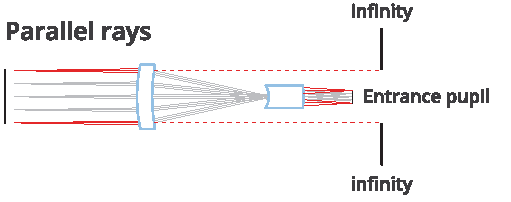
\includegraphics[width=0.6\textwidth]{telecentric-optical-system.pdf}
	\caption{物方远心光学系统}
	\label{fig:telecentric-optical-system}
\end{figure}